% withpage: ページ番号をつける (著者確認用)
% english: 英語原稿用フォーマット
\documentclass{ipsjprosym}
%\documentclass[withpage,english]{ipsjprosym}

\usepackage[dvips]{graphicx}
\usepackage{latexsym}

\begin{document}

% Title, Author %%%%%%%%%%%%%%%%%%%%%%%%%%%%%%%%%
\title{ATS言語を使って不変条件をAPIに強制する}

\affiliate{METASEPI}{METASEPI DESIGN}

\author{岡部 究}{Kiwamu Okabe}{METASEPI}[kiwamu@debian.or.jp]

\begin{abstract}
概要(400字程度)○○○○○○○○○○○○○○○○○○○○○○○○○○○○○○○
○○○○○○○○○○○○○○○○○○○○○○○○○○○○○○○○○○○○○○○○
○○○○○○○○○○○○○○○○○○○○○○○○○○○○○○○○○○○○○○○○
○○○○○○○○○○○○○○○○○○○○○○○○○○○○○○○○○○○○○○○○
○○○○○○○○○○○○○○○○○○○○○○○○○○○○○○○○○○○○○○○○
○○○○○○○○○○○○○○○○○○○○○○○○○○○○○○○○○○○○○○○○
○○○○○○○○○○○○○○○○○○○○○○○○○○○○○○○○○○○○○○○○
○○○○○○○○○○○○○○○○○○○○○○○○○○○○○○○○○○○○○○○○
○○○○○○○○○○○○○○○○○○○○○○○○○○○○○○○○○○○○○○○○
○○○○○○○○○○○○○○○○○○○○○○○○○○○○○○○○○○○○○○○○
\end{abstract}

\begin{jkeyword}
ATS, 関数型言語, 依存型, 線形型, 組込開発
\end{jkeyword}

\maketitle

% Body %%%%%%%%%%%%%%%%%%%%%%%%%%%%%%%%%
\section{はじめに}
\section{既存の組込開発手法の問題}
\section{ATS言語とは}

\begin{figure}[h]
\centering
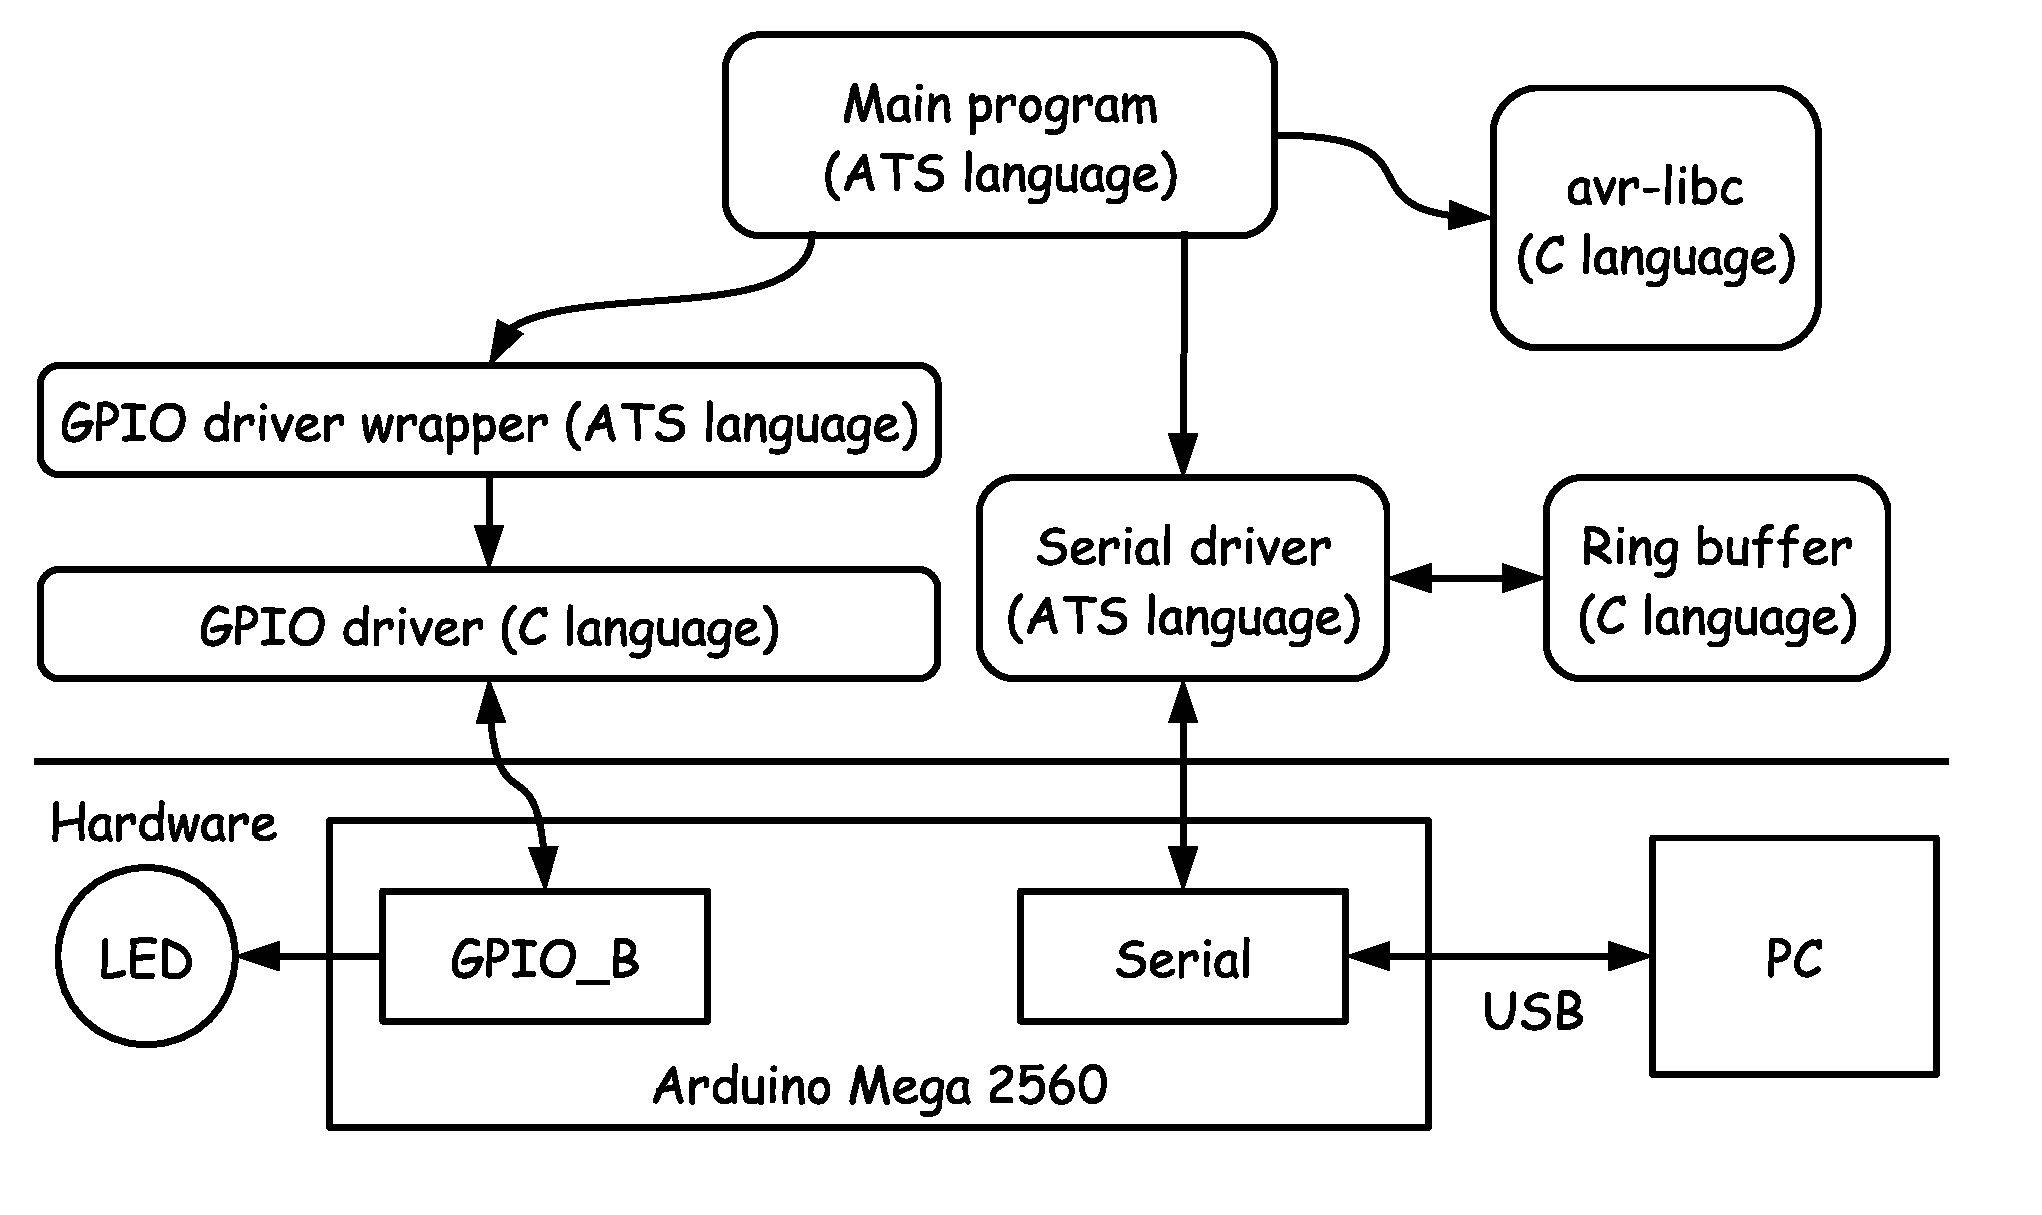
\includegraphics[width=75mm]{draw/demo_ats_arduino.eps}
\caption{xxx}
\label{fig:demo_ats_arduino}
\end{figure}

\begin{figure}[h]
\centering
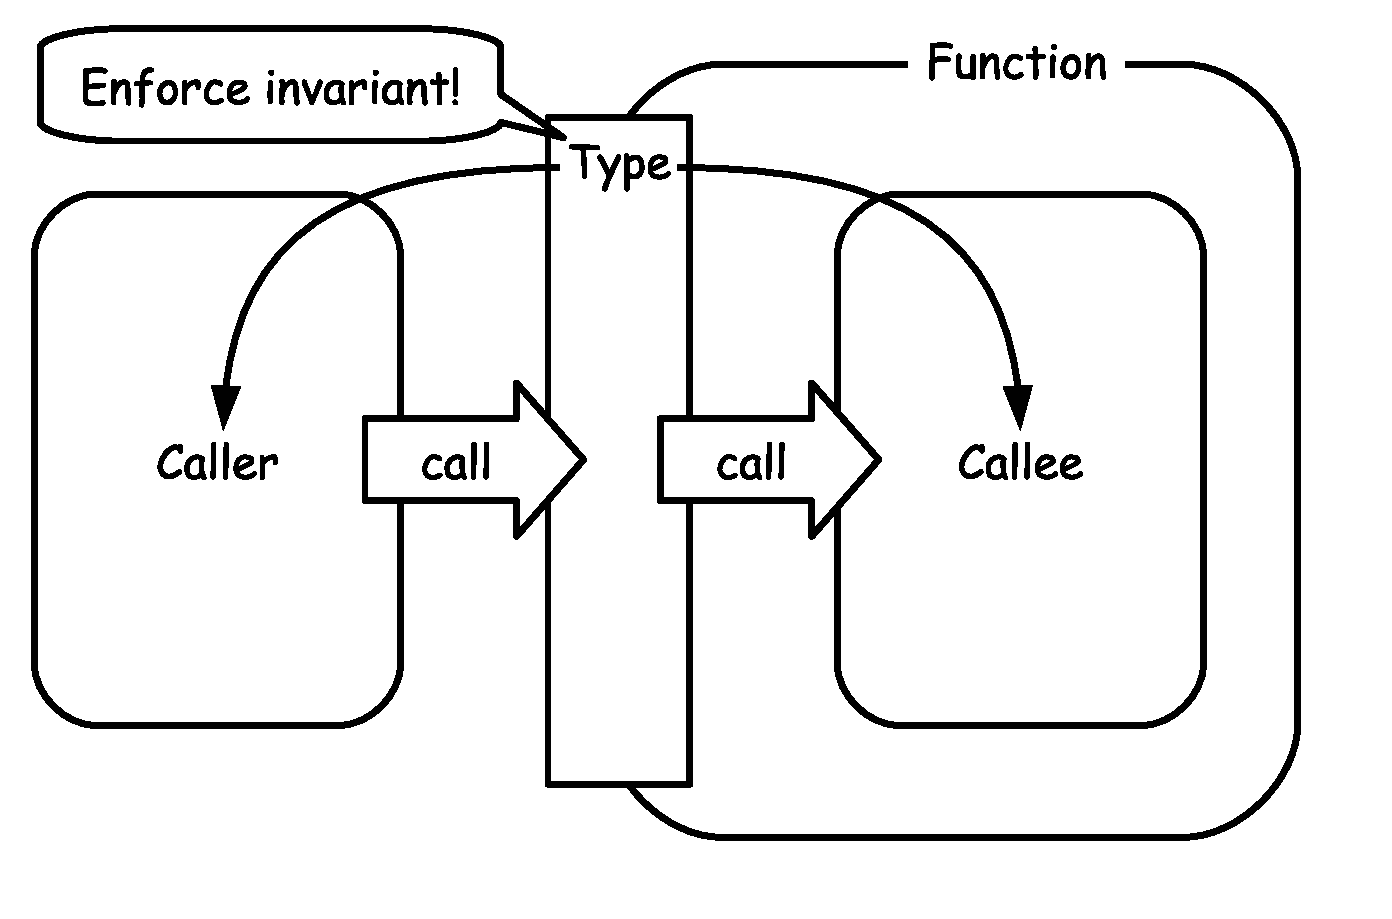
\includegraphics[width=75mm]{draw/enforce_invariant.eps}
\caption{xxx}
\label{fig:enforce_invariant}
\end{figure}

\begin{figure}[h]
\centering
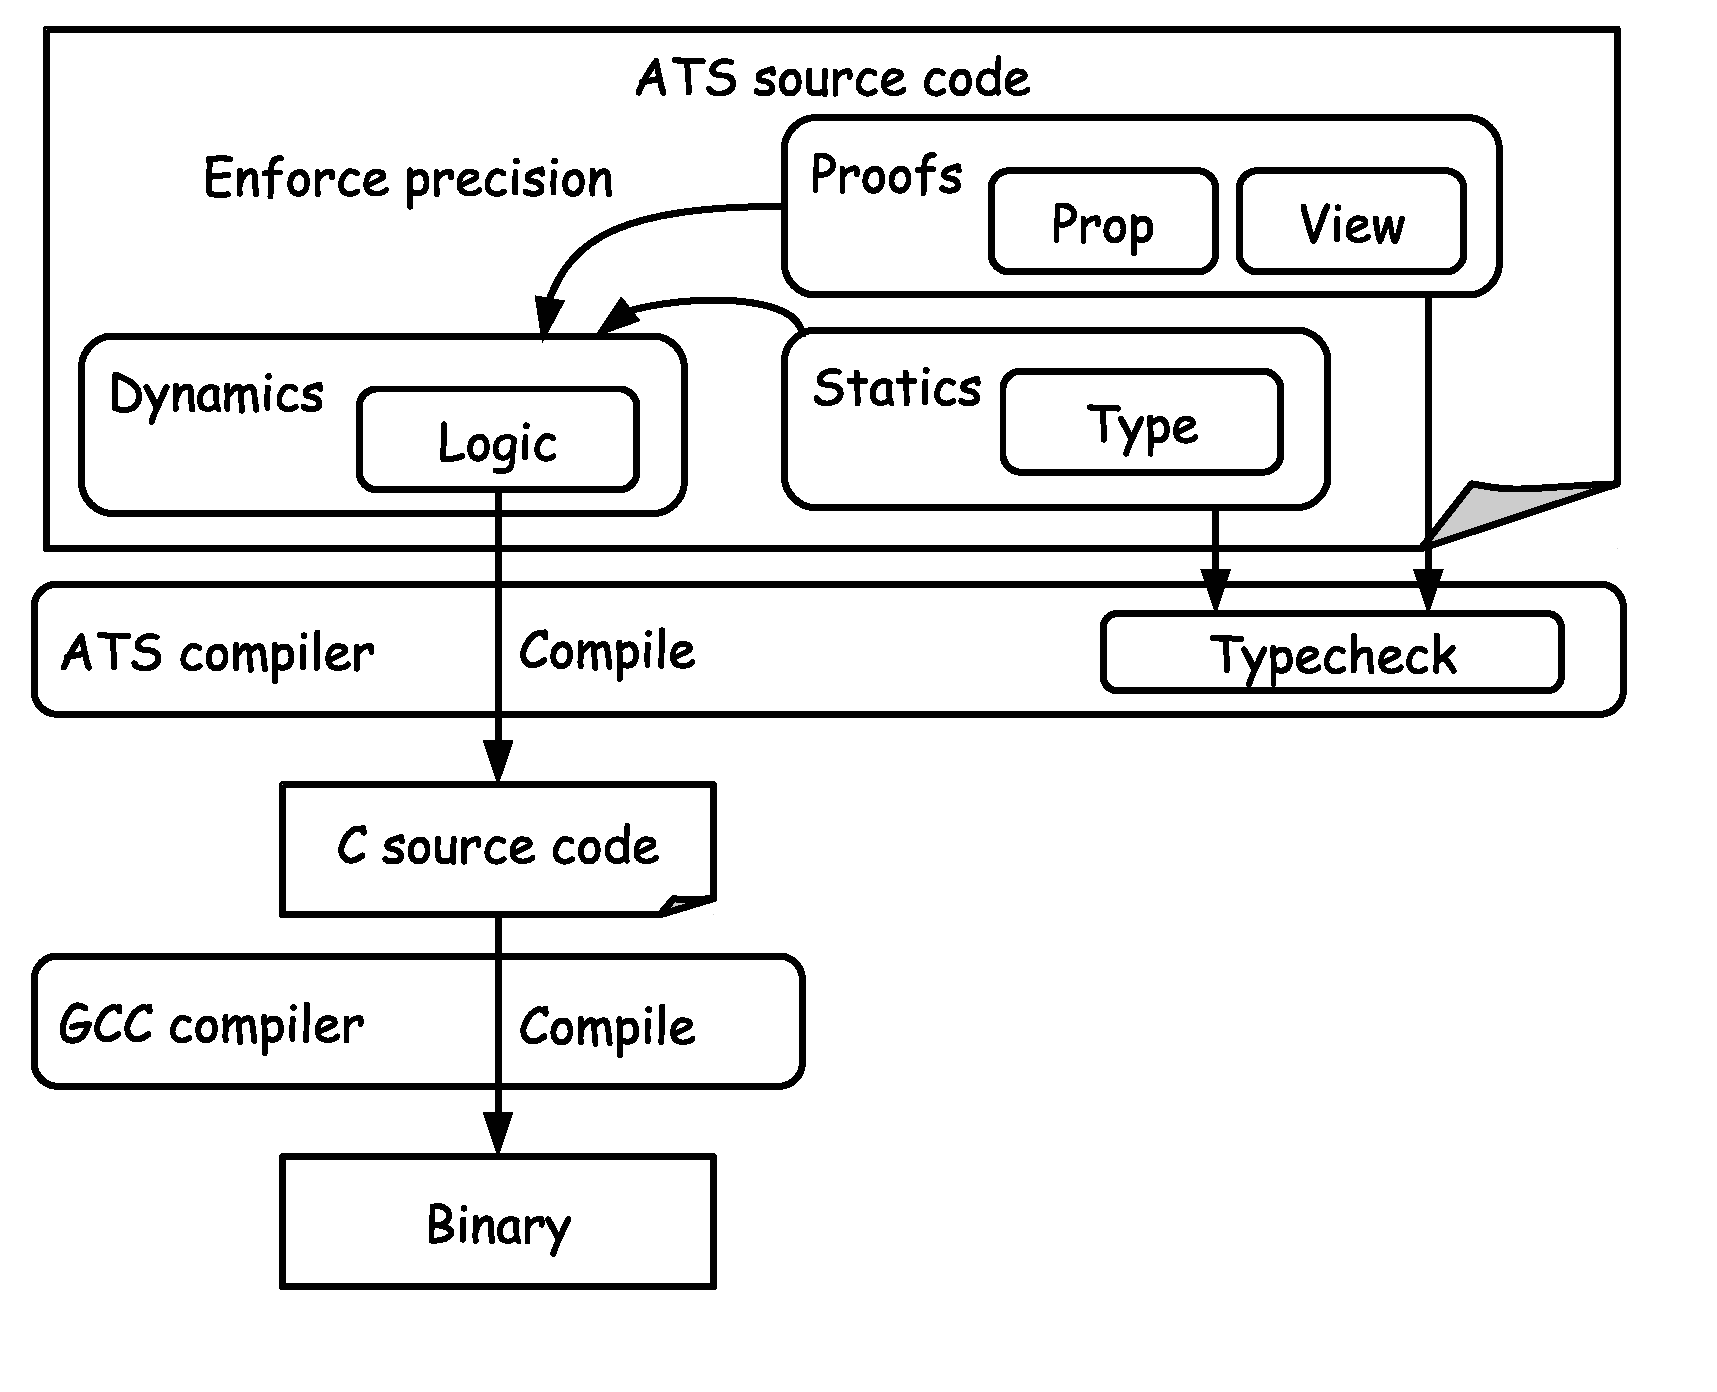
\includegraphics[width=75mm]{draw/flow.eps}
\caption{xxx}
\label{fig:flow}
\end{figure}

\begin{figure}[h]
\centering
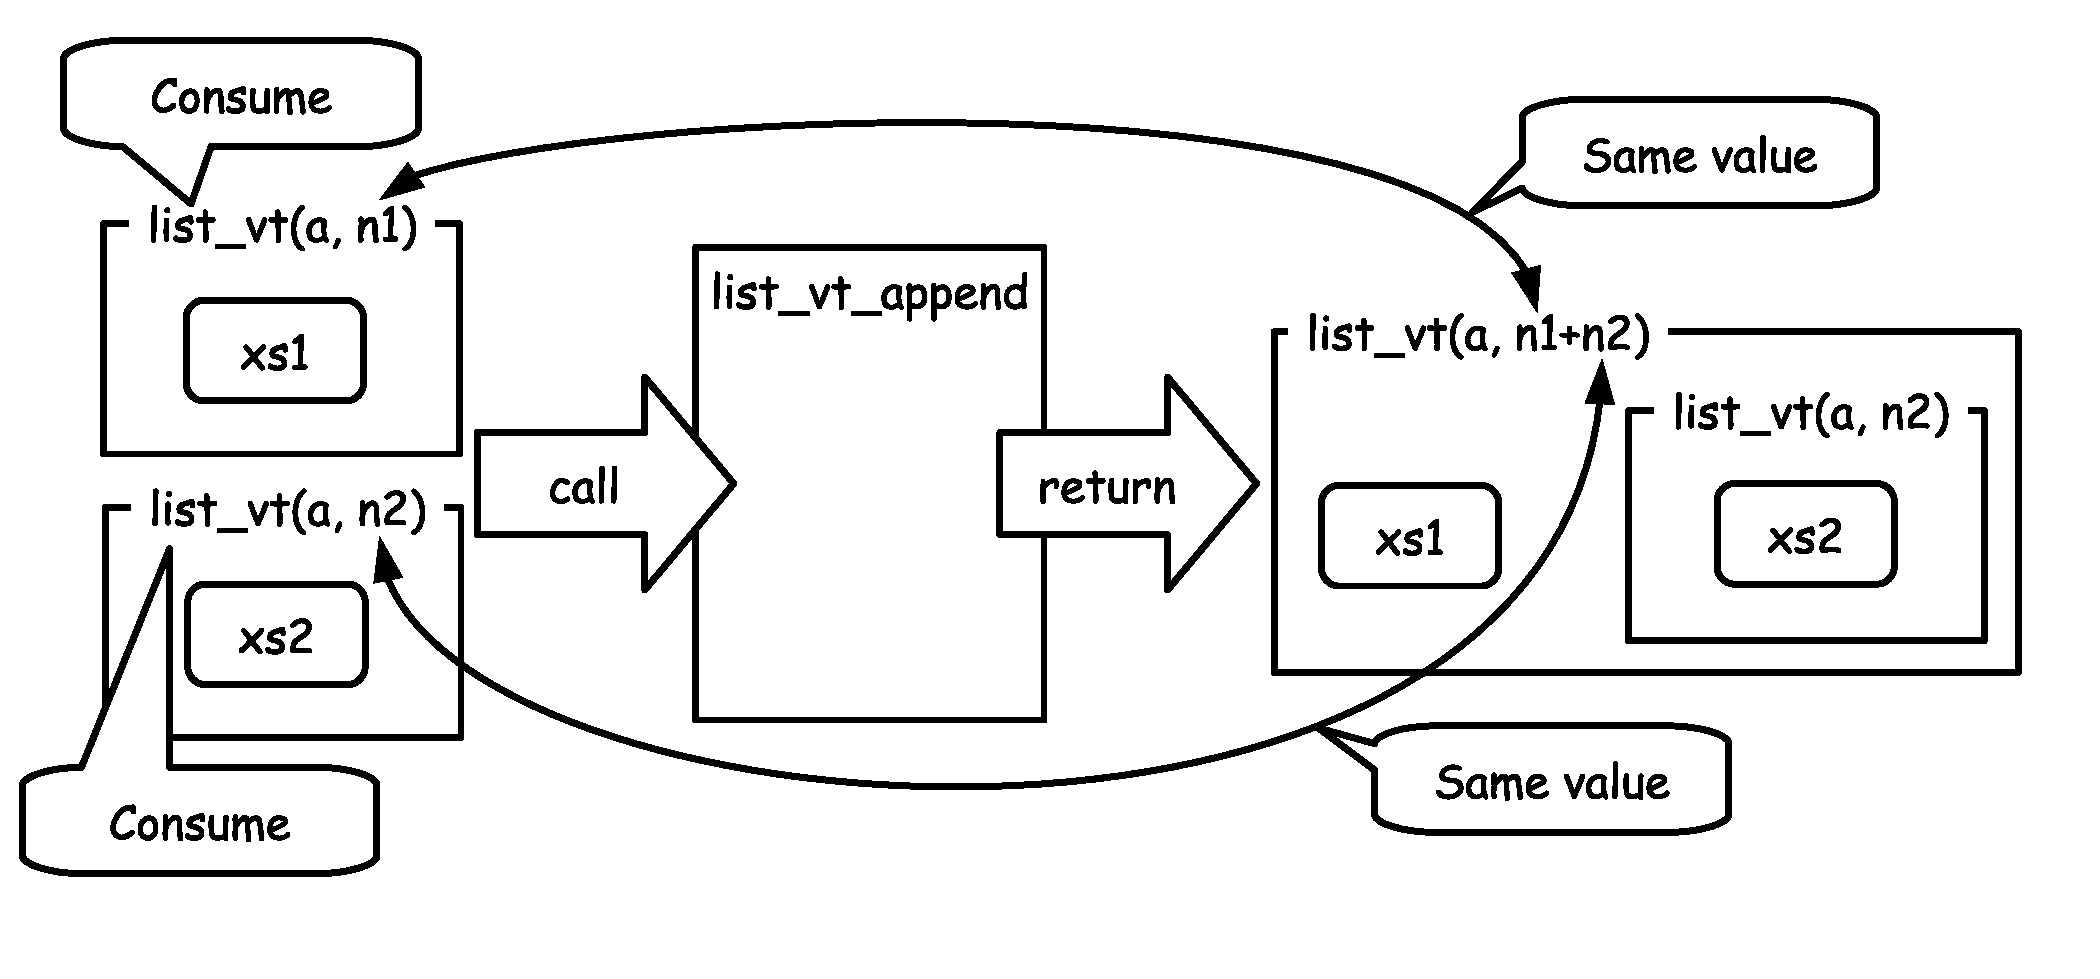
\includegraphics[width=75mm]{draw/list_vt_append.eps}
\caption{xxx}
\label{fig:list_vt_append}
\end{figure}

\begin{figure}[h]
\centering
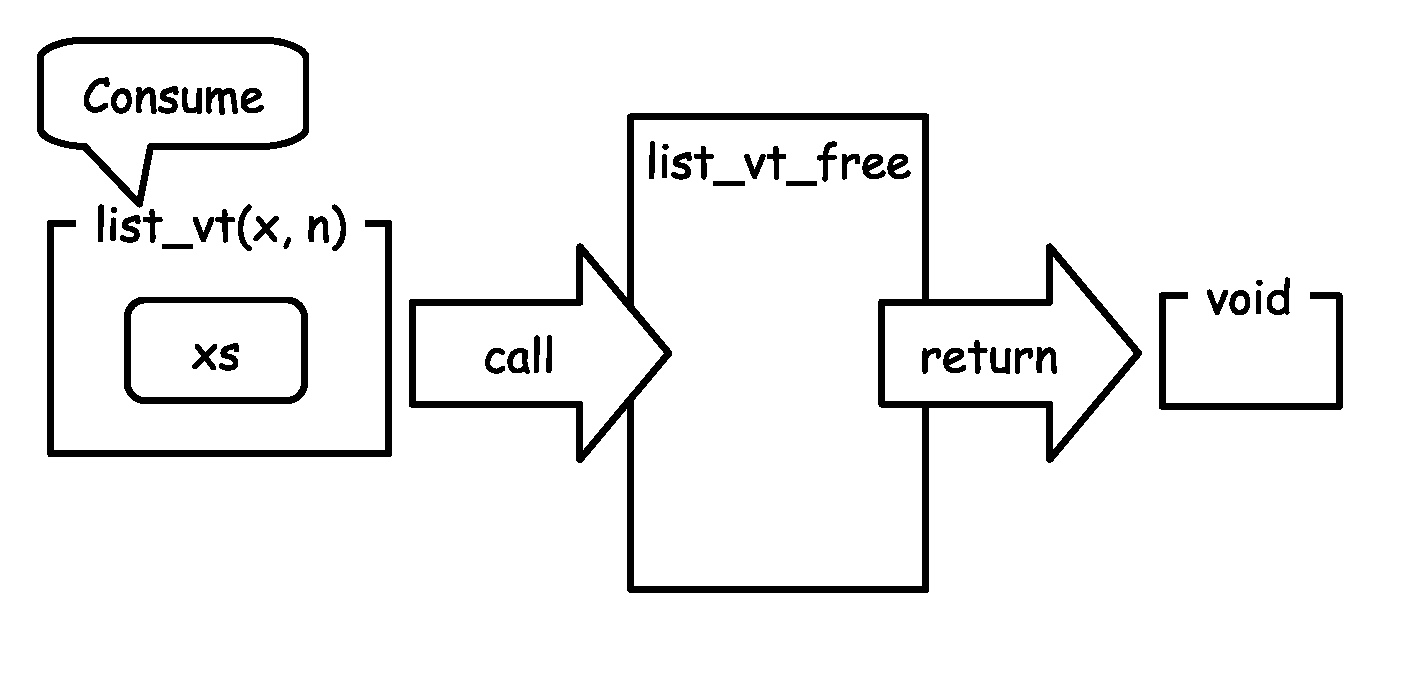
\includegraphics[width=75mm]{draw/list_vt_free.eps}
\caption{xxx}
\label{fig:xxx}
\end{figure}

\begin{figure}[h]
\centering
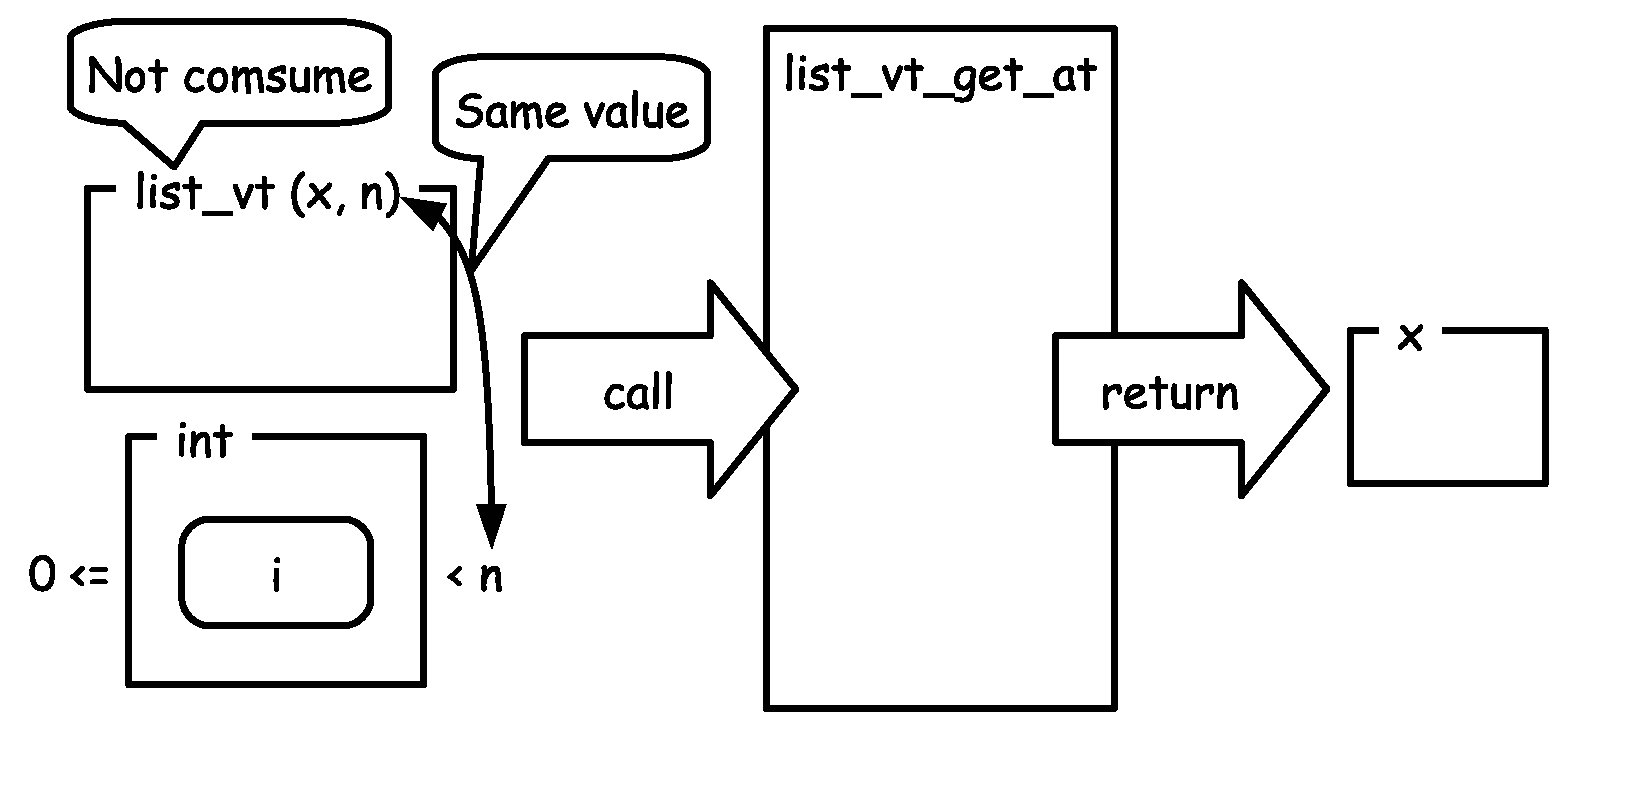
\includegraphics[width=75mm]{draw/list_vt_get_at.eps}
\caption{xxx}
\label{fig:xxx}
\end{figure}

\begin{figure}[h]
\centering
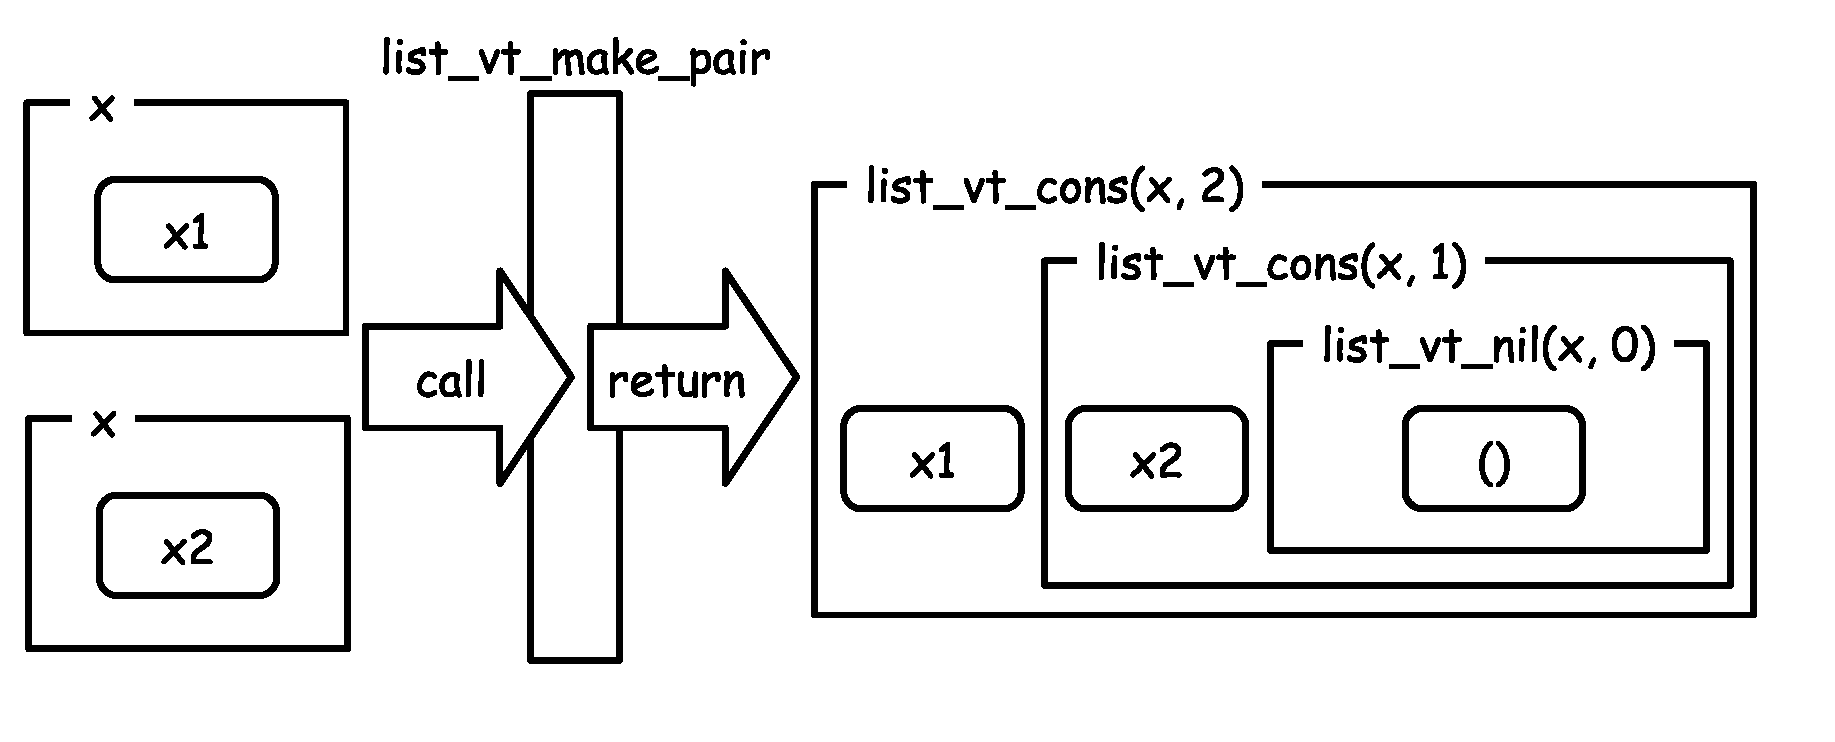
\includegraphics[width=75mm]{draw/list_vt_make_pair.eps}
\caption{xxx}
\label{fig:xxx}
\end{figure}

\begin{figure}[h]
\centering
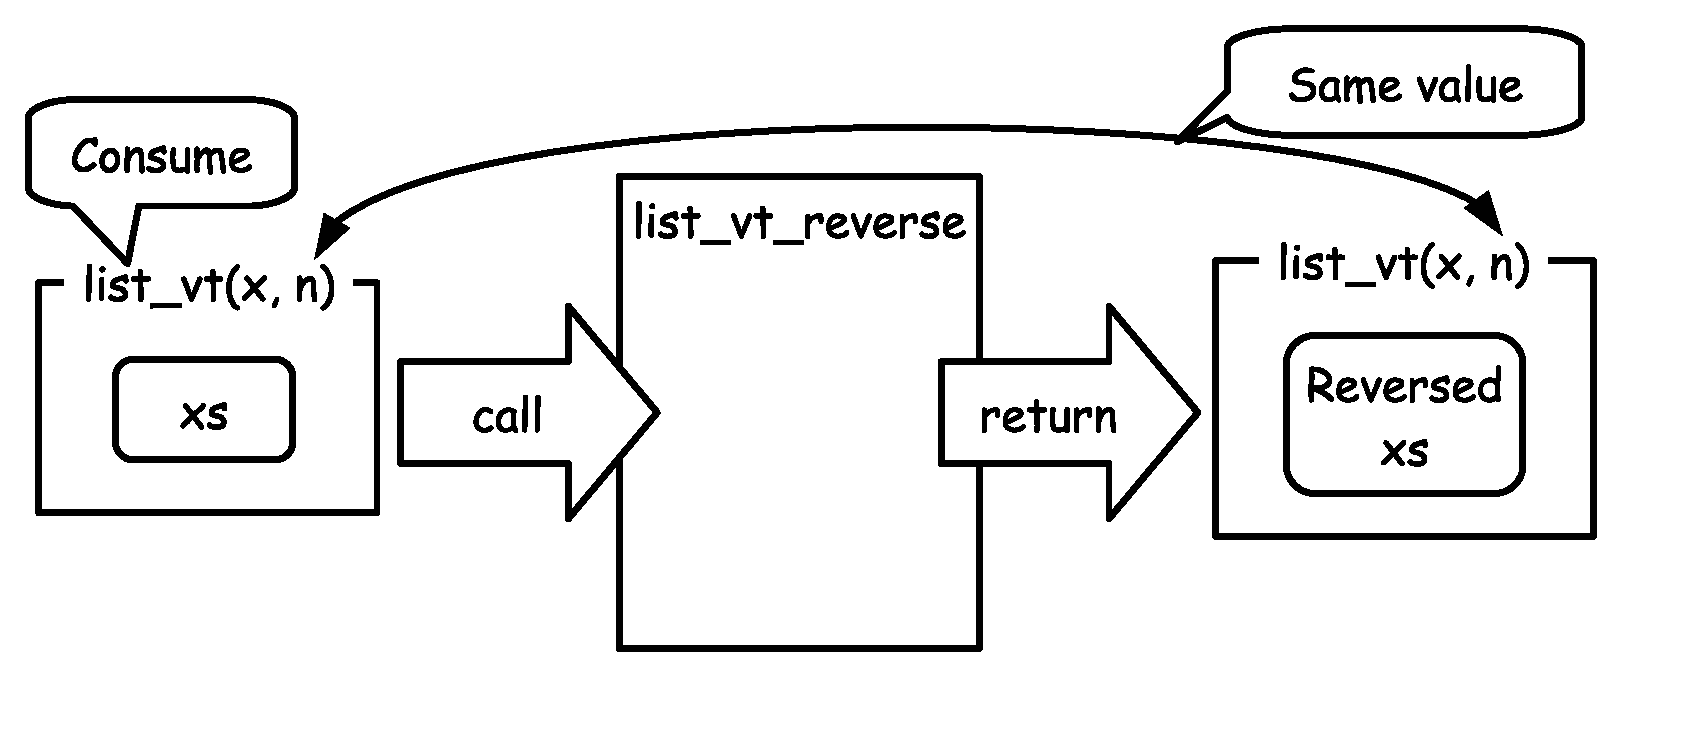
\includegraphics[width=75mm]{draw/list_vt_reverse.eps}
\caption{xxx}
\label{fig:xxx}
\end{figure}

\begin{figure}[h]
\centering
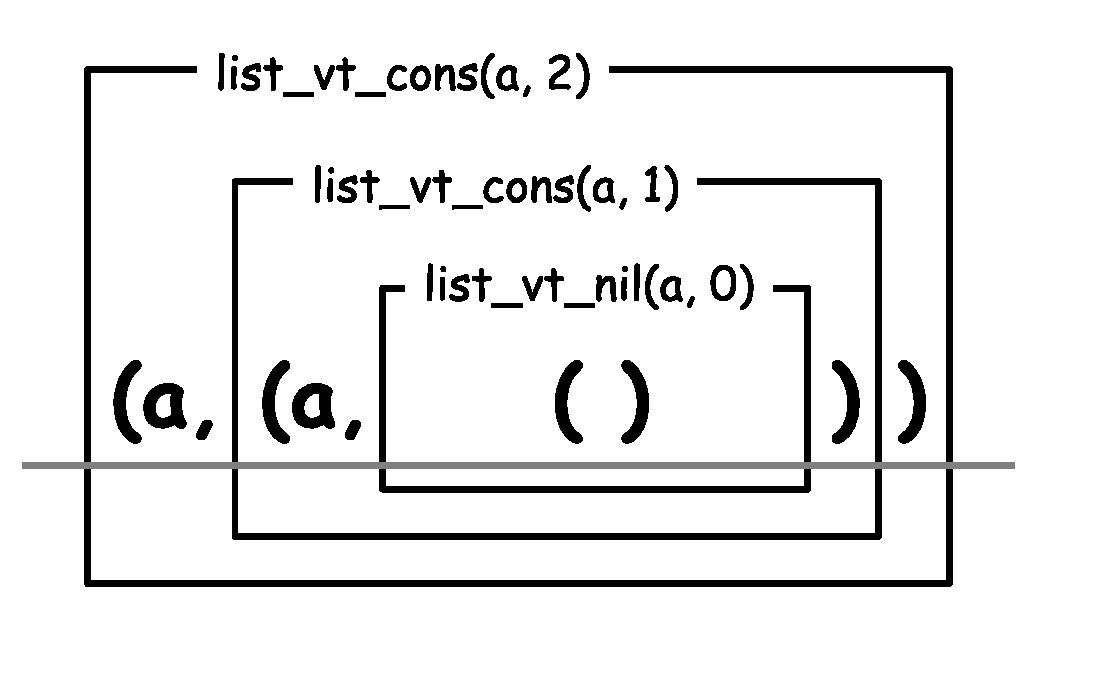
\includegraphics[width=75mm]{draw/list_vt_type.eps}
\caption{xxx}
\label{fig:xxx}
\end{figure}

\section{ATSによる組込開発手法と考察}
\section{結論と今後の課題}

\begin{acknowledgment}
ATS言語に関して助言をくれたボストン大学の准教授であるHongwei XiとATSコミュニティに感謝する。
\end{acknowledgment}

% BibTeX を使用する場合 %%%%%%%%%%%%%%%%%%%%%%%%%%%%%%%%%
% \bibliographystyle{ipsjsort}
% \bibliography{ref}

% BibTeX を使用しない場合
\begin{thebibliography}{9}
 \bibitem{latex} 奥村晴彦, 黒木裕介: \textbf{LaTeX2e美文書作成入門}. 技術評論社, 2013.
\end{thebibliography}

\begin{QandA}
\item[A] 線形型にvalで別名を作るとどうなるのか?
\item[岡部] 消費される。以下の例を付記する。

\begin{verbatim}
(* コンパイルNG: let valでも線形型が消費されてしまう *)
#include "share/atspre_staload.hats"
implement main0 () = {
  val l1 = list_vt_make_pair<int> (1, 2)
  val l2 = l1
  val () = let val l3 = l2
           in println! l3 end
  val () = free l2
}

(* コンパイルOK: valで線形型が消費される *)
#include "share/atspre_staload.hats"
implement main0 () = {
  val l1 = list_vt_make_pair<int> (1, 2)
  val l2 = l1
  val () = println! l2
  val () = free l2
}
\end{verbatim}

\item[B] リングバッファをATSで書くのは難しいのか?
\item[岡部] 公式ドキュメントに例があるぐらいなので、リングバッファ自体は簡単。しかし、スレッドセーフ化や再入可能にするのはそれなりに難しい。
\item[C] マルチスレッドを生かしたプログラミングをするにはどうすれば良いか?
\item[岡部] セッションのようなものを作る。例えばmutexのロックと開放では、その間にセッションが存在すると考えることができる。セッションの間は静的な型を効果的に使うことができる。
\item[D] ATSに辿りつくまでのMetasepiプロジェクトの歴史について
\item[岡部] ATSを使ったイテレーションは2番目。1番目ではHaskell言語とjhcコンパイラを使っていた。Haskellの欠点は、メモリ領域の扱いがルーズ、マシン表現と言語表現にギャップがあること。ATSの欠点は、抽象化の機能が弱いこと。
\end{QandA}

\end{document}
